\section{Empirical Application}\label{sec:empirical}

\subsection{Data}

To evaluate the model in a realistic environment, we use a large cross-section of assets and a high-dimensional set of news-based predictors.
Our sample consists of the daily returns of all stocks that were continously listed on the New York Stock Exchange (NYSE) between 2010 and 2017.
As predictors, we use the 180 daily news topic attention series constructed by \citet{Bybee2021} from the full text of the \textit{Wall Street Journal} using an unsupervised Latent Dirichlet Allocation (LDA) model.
The LDA assigns each article a vector of topic proportions, which \citet{Bybee2021} aggregate to the daily frequency to measure media attention across a broad set of business, economic, political, and social topics.
A complete list of all 180 topics is provided in Table \ref{tab:news_topics}.
We supplement these with 10 daily macro-financial time series — the Fed Funds rate, the 10-year and 3-month Treasury yields, the VIX, the Financial Stress Index, the High Yield spread, the Trade-Weighted USD index, WTI crude oil, the 10-year breakeven inflation rate, and the USD/JPY exchange rate — which agents may plausibly use alongside news-topic signals when forming beliefs about return predictability.
The resulting predictor set of 190 series is highly heterogeneous, with little theoretical guidance as to which variables are relevant.
In this environment, we argue, it is natural for agents to rely on LASSO-based learning to identify the most informative signals.

We use innovations rather than levels for all 190 predictors, since both news attention and macro-financial series are highly persistent and their levels primarily capture slow-moving trend components.
To isolate unexpected changes in information, we estimate an AR($p$) process for each series, where the lag length $p$ is selected using the Akaike Information Criterion (AIC), and define $X_t$ as the corresponding residuals.
Consistent with the model, we work with log returns, defined as $r_{i,t} = \log(R_{i,t})$, where $R_{i,t}$ denotes the gross return of stock $i$ on day $t$.
The final sample contains returns of 1{,}620 stocks and 190 predictors over 1{,}889 trading days.
Table~\ref{tab:summary_stats} reports summary statistics of our data.

\begin{table}[H]
\centering
\caption{Summary Statistics}
\label{tab:summary_stats}

\begin{tabularx}{\textwidth}{@{}>{\small}Xccccccr@{}}
\toprule
Variable & Mean & Std.\ Dev. & Min & Max & Skewness & Kurtosis & $N$ \\
\midrule
Log return 
& 0.000 & 0.021 & $-$1.964 & 2.051 & $-$0.587 & 101.917 & 3{,}060{,}180 \\
\midrule
Topic level 
& 0.006 & 0.004 & 0.000 & 0.116 & 3.662 & 33.361 & 340{,}020 \\
Topic innovation 
& 0.000 & 0.003 & $-$0.054 & 0.062 & 1.885 & 16.019 & 339{,}840 \\
\bottomrule
\end{tabularx}

\medskip
\begin{minipage}{\textwidth}
\footnotesize
\textit{Note:} The table reports summary statistics for daily log returns
$r_{i,t}=\log(R_{i,t})$ of NYSE-listed stocks from 2010--2017 and for news-topic
attention measures constructed following \citet{Bybee2021}.
Topic attention innovations are defined as residuals from topic-specific AR(p)
regressions estimated over the full sample, where the lag length $p$ is selected using the Akaike Information Criterion (AIC).
\end{minipage}
\end{table}


\subsection{Estimation Strategy}

Our theory has two core components: (i) a misspecified PLM through which agents form beliefs about return predictability, and (ii) an ALM that maps these beliefs into realized returns. 
Because neither the agents nor the econometrician observe the true data-generating process for returns, our empirical strategy mirrors the agents’ learning problem.
We begin by estimating the PLM as in the model, while introducing some modifications to make the framework empirically implementable.


First, we assume that agents estimate the PLM using a rolling window of fixed length rather than geometrically declining weights, which is more in line with standard econometric practices when dealing with potential time-varying parameters and allow us to closely mirror
the design of \cite{Chinco2019}.
Second, we endow agents with a full LASSO regression rather than the soft-thresholding approximation used in the theoretical analysis.
As already remarked, the soft-thresholding operator is exactly equivalent to LASSO when regressors are orthonormal.
Instead, we allow regressors to be approximatly uncorrelated, which is a weaker but more realistic condition.
Third, we allow for lags of the regressors to enter the PLM, by stacking $n$ lags of each predictor innovation as potential predictors.
This extension captures the possibility that agents consider delayed effects of news and macro signals on returns.
Accordingly, equation~(\ref{eq:lasso_from_ols}) need not hold exactly, but should provide a close approximation.
Consistent with this assumption, Figure~\ref{fig:corr_heatmap} in Appendix~\ref{app:tab_figures} shows that predictor innovations are close to contemporaneously uncorrelated, while Table~\ref{tab:cross_lag_correlations} documents that cross-lag correlations in the time series are also small.
At each date \(t\), the information set consists of \(k=190\) predictor innovations (180 topic-attention and 10 macro-financial series). Let
\(x_t \in \mathbb{R}^{k}\) denote the vector of innovations at time \(t\), with element
\(x_{j,t}\) corresponding to predictor \(j \in \{1,\ldots,k\}\).
For a rolling window of length \(s\), define the regressor matrix by stacking past topic
vectors row-wise,
\begin{equation}
X_t \in \mathbb{R}^{s \times k}
\equiv
\begin{bmatrix}
x_{t-s}^\top \\
x_{t-s+1}^\top \\
\vdots \\
x_{t-1}^\top
\end{bmatrix},
\qquad
r_{i,t+1} \in \mathbb{R}^{s}
\equiv
\begin{bmatrix}
r_{i,t-s+1} \\
r_{i,t-s+2} \\
\vdots \\
r_{i,t}
\end{bmatrix}.
\end{equation}
Each row of \(X_t\) is a \(1 \times k\) vector of topic innovations observed at a given date,
while each column tracks the time series of innovations for a given topic over the window.

For each stock \(i\) and each window ending at \(t-1\), the agent estimates a LASSO
coefficient vector
\begin{equation}
\beta_{i,t} \in \mathbb{R}^{k},
\end{equation}
so that beliefs are indexed by both time and topic. Equivalently, the collection
\(\{\beta_{i,t}\}_t\) defines a stock-specific, time-varying belief process, where the
\(j\)-th element \(\beta_{i,t}^{(j)}\) measures the perceived predictive content of topic \(j\)
for stock \(i\) at date \(t\).
The empirical perceived law of motion (PLM) for log returns is therefore
\begin{equation}\label{eq:empirical_plm}
r_{i,t+1} = X_t \beta_{i,t} + \eta_{i,t+1},
\end{equation}
where \(X_t \beta_{i,t} \in \mathbb{R}^{s}\) denotes the vector of fitted within-window returns
implied by the \(k\)-dimensional belief vector at date \(t\).
Applying this procedure sequentially yields a time-varying sequence of belief parameters
\(\{\beta_{i,t}\}\) for each stock.

Using the estimated belief path, we then estimate the empirical actual law of motion
(ALM) implied by the asset-pricing equation.\footnote{While the theoretical model implies
zero unconditional mean log returns under our maintained assumptions, the empirical
specification includes an intercept to absorb average return components not captured by
the model.}
\begin{equation}\label{eq:empirical_alm}
r_{i,t+1}
= c_i
+ \log\!\left(1 - \kappa_i e^{x_t^\top \beta_{i,t}}\right)
- \log\!\left(1 - \kappa_i e^{x_{t+1}^\top \beta_{i,t+1}}\right)
+ \eta_{i,t+1},
\end{equation}
where \(x_t^\top \beta_{i,t}\) is scalar because \(x_t, \beta_{i,t} \in \mathbb{R}^{k}\).
The stock-specific parameter \(\kappa_i\) is estimated by nonlinear least squares.


Prior to implementing our estimation strategy, we fix the rolling window length and calibrate only the LASSO penalty ($\lambda$).
Throughout the empirical analysis, we use one lag of the predictor innovations.
We set the baseline window to $s=252$ trading days, corresponding to one calendar year of daily data.\footnote{The choice of 252 trading days is motivated by the natural information horizon of a calendar year: corporate earnings cycles, annual reports, and macroeconomic policy reviews all operate at this frequency, making it a reasonable upper bound on how long a piece of news remains statistically relevant for forecasting returns.}
In our setting, window length is a proxy for memory length: how far back information remains relevant for forecasting next-day returns.
This choice also aligns with standard annual governance and model review cycles in practice.

Because the penalty is not known ex ante, we select $\lambda$ via a cross-sectional hold-out procedure, reserving 20\% of stocks as a tuning set while the remaining 80\% form the estimation sample.
The standard approach in the literature is to cross-validate on a predictive loss such as MSE or out-of-sample $R^2$ \citep{Chinco2019, Gu2020, Feng2020}.
For our purposes, however, the object of interest is not predictive accuracy per se but the identification of $\kappa$ which would confirm the validity of our CMCE model.
So the correct penalty should produce sparse, non-degenerate beliefs that yield a statistically significant second-stage estimate.
We show in Appendix~\ref{app:oracle} that a composite objective that combines the first-stage in-sample fit with the second-stage significance of $\kappa$ performs well in recovering the true penalty in a simulated environment.
The optimization based on this objective yields $\lambda = 3.224 \times 10^{-3}$, which is then fixed and applied across all estimation stocks.


\subsection{Results}

We then evaluate the model in the cross-section.
For each stock, we estimate the PLM in equation~(\ref{eq:empirical_plm}) using a rolling-window LASSO.
This procedure delivers a time series of belief coefficients $\{\beta_{i,t}\}$ and corresponding one-step-ahead forecasts, which we summarize in Table~\ref{tab:summary_stats_lasso}.

\begin{table}[H]
\centering
\caption{Summary Statistics of LASSO Estimation Results}
\label{tab:summary_stats_lasso}
\begin{tabularx}{\textwidth}{@{}>{\small}Xccccccc@{}}
\toprule
 & mean & std & median & min & max & p05 & p95 \\
\midrule
In-sample $R^2$   & 0.0249 & 0.0416 & 0.0071 & $-$0.0073 & 0.2790 & $-$0.0040 & 0.1124 \\
Out-of-sample $R^2$ & $-$0.0115 & 0.0234 & $-$0.0035 & $-$0.3677 & 0.0054 & $-$0.0488 & $-$0.0001 \\
Selection rate    & 0.0222 & 0.0350 & 0.0071 & 0.0000 & 0.2464 & 0.0000 & 0.0971 \\
\bottomrule
\end{tabularx}
\medskip
\begin{minipage}{\textwidth}
\footnotesize
\textit{Note:} The table reports summary statistics across the 1,296 estimation stocks for the first-stage LASSO in-sample $R^2$, computed within each rolling window and averaged over windows, the first-stage out-of-sample $R^2$, computed from the sequence of one-step-ahead LASSO forecasts evaluated against realised (demeaned) returns with the zero-forecast as benchmark, and the average LASSO selection rate (fraction of predictor-window cells with a non-zero coefficient).
\end{minipage}
\end{table}

Table~\ref{tab:summary_stats_lasso} shows that the in-sample $R^2$ is small but positive, indicating that the LASSO learning rule fits the return process within windows.
The out-of-sample $R^2$ is near zero.
The patterns are consistent with our theory: agents perceive transient predictability in-sample, but it does not persist out-of-sample.
This is a direct implication of the CMCE condition $\beta^* = 0$.
The median selection rate is 0.71\%, confirming that beliefs are sparse.
Approximately 40\% of stocks have selection rates below 0.3\%, implying that the LASSO never selects any predictor for these stocks.
This is also consistent with the model: for stocks whose return variance is small relative to the penalty level, the LASSO correctly infers that there is insufficient evidence to support a non-zero belief vector, leaving $f_t = 0$ throughout.

With the LASSO-estimated belief sequence $\{\beta_{i,t}\}$ in hand, we turn directly to the main coefficient of interest and estimate the parameter $\kappa_{i}$ implied by the ALM by applying nonlinear least squares to equation~(\ref{eq:empirical_alm}).
Identification relies on time-series variation in agents’ beliefs about return predictability, as captured by fluctuations in $X_t \beta_{i,t}$, and on the corresponding variation in realized returns.
Intuitively, $\kappa_{i}$ is pinned down by how changes in expected returns translate into realised returns through the nonlinear asset-pricing equation.
A significant $\kappa$ indicates that the non-linear ALM has explanatory power over a benchmark where returns are unpredictable, and we view it as an empirical test of the CMCE equilibrium being present in the data.
Of the 782 estimation stocks with non-zero LASSO selection, for which $f_t$ exhibits sufficient time-series variation to identify $\kappa$, 13.2\% have a statistically significant estimate at the 5\% level.
Table~\ref{tab:summary_stats_stage2} summarises the estimation results for these stocks.

\begin{table}[H]
\centering
\caption{Second-Stage Estimation: Summary Statistics}
\label{tab:summary_stats_stage2}
\begin{tabularx}{\textwidth}{@{}>{\small}Xccccccc@{}}
\toprule
 & mean & std & median & min & max & p05 & p95 \\
\midrule
In-sample $R^2$        & 0.0026 & 0.0017 & 0.0022 & 0.0009 & 0.0102 & 0.0011 & 0.0060 \\
Out-of-sample $R^2$    & $-$0.0179 & 0.0607 & $-$0.0019 & $-$0.4139 & 0.0289 & $-$0.0876 & 0.0068 \\
$\hat{\kappa}$         & 0.2938 & 0.1270 & 0.2707 & 0.0877 & 0.6879 & 0.1149 & 0.5193 \\
$t$-statistic of $\hat{\kappa}$ & 2.9634 & 1.2818 & 2.5270 & 1.9684 & 10.6818 & 1.9923 & 5.2329 \\
\bottomrule
\end{tabularx}
\medskip
\begin{minipage}{\textwidth}
\footnotesize
\textit{Note:} The table reports summary statistics across the 103 estimation stocks (13.2\% of the 782 with non-zero LASSO selection) for which $\hat\kappa$ is statistically significant at the 5\% level and the NLS estimate is non-degenerate.
In-sample $R^2$ is the second-stage NLS fit evaluated on the full time series.
Out-of-sample $R^2$ is computed from one-step-ahead forecasts of the ALM evaluated against realised returns with the zero-forecast as benchmark.
$\hat{\kappa}$ is the estimated belief-feedback parameter and its $t$-statistic is computed from the NLS sandwich standard error.
\end{minipage}
\end{table}

We then move to analyze wether the results of the estimation on empirical data are consistent with the theory developed in the previous sections.
First, we test the cross-sectional implication in Proposition~\ref{prop:LASSO_estimate} that stocks with higher idiosyncratic volatility should exhibit more frequent selection.
Figure~\ref{fig:avg_select} plots, for each stock, the mean LASSO selection rate against its idiosyncratic volatility $\hat{\sigma}_i$, measured as the standard deviation of Stage-2 residuals.
Stocks with a statistically significant $\hat{\kappa}$ estimate (at the 5\% level) are highlighted in red.
The relationship is strongly positive and convex: stocks with low idiosyncratic volatility are almost never selected, while the most volatile stocks are selected in around 15\% of rolling windows.

\begin{figure}[h]
    \centering
    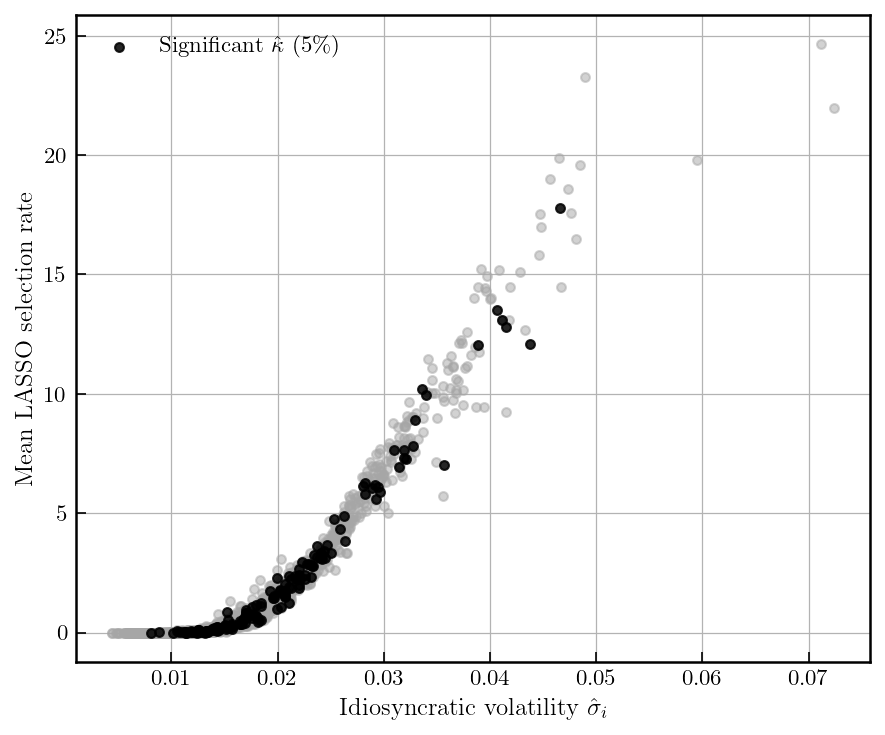
\includegraphics[width=0.7\textwidth]{scatter_idio_vol_selection_r2.png}
    \caption{Mean LASSO Selection Rate vs.\ Idiosyncratic Volatility}
    \label{fig:avg_select}
\end{figure}

We view these patterns as evidence in favor of our proposed learning rule.
An agent applying LASSO-based learning to the data would find the rule attractive ex ante, because it delivers nontrivial in sample fit, even though its out of sample performance is weak.
Consistent with our theory, perceived predictability is episodic, so at any point in time only a subset of stocks is viewed as predictable and, conditional on selection, beliefs are sparse and concentrated on a few predictors.
Taken together, these results match the model’s predictions and mirror recent evidence that return predictability arises in short lived, shifting pockets rather than as a stable forecasting relation \citep{Chinco2019}.




Having established the explanatory power of the ALM, we next explore the underlying properties of the estimated beliefs that drive these results.
First, we document that perceived predictability is concentrated in a few signals when it arises.
Figure~\ref{fig:percent_active} plots the average number of selected predictors per stock over time, as well as shaded areas corresponding to the 5th and 95th percentiles across stocks.
Out of the whole possible 190 predictors, the share that is selected is small, indicating that when agents believe in predictability, they typically attribute it to only a small subset of available signals.

\begin{figure}[h]
    \centering
    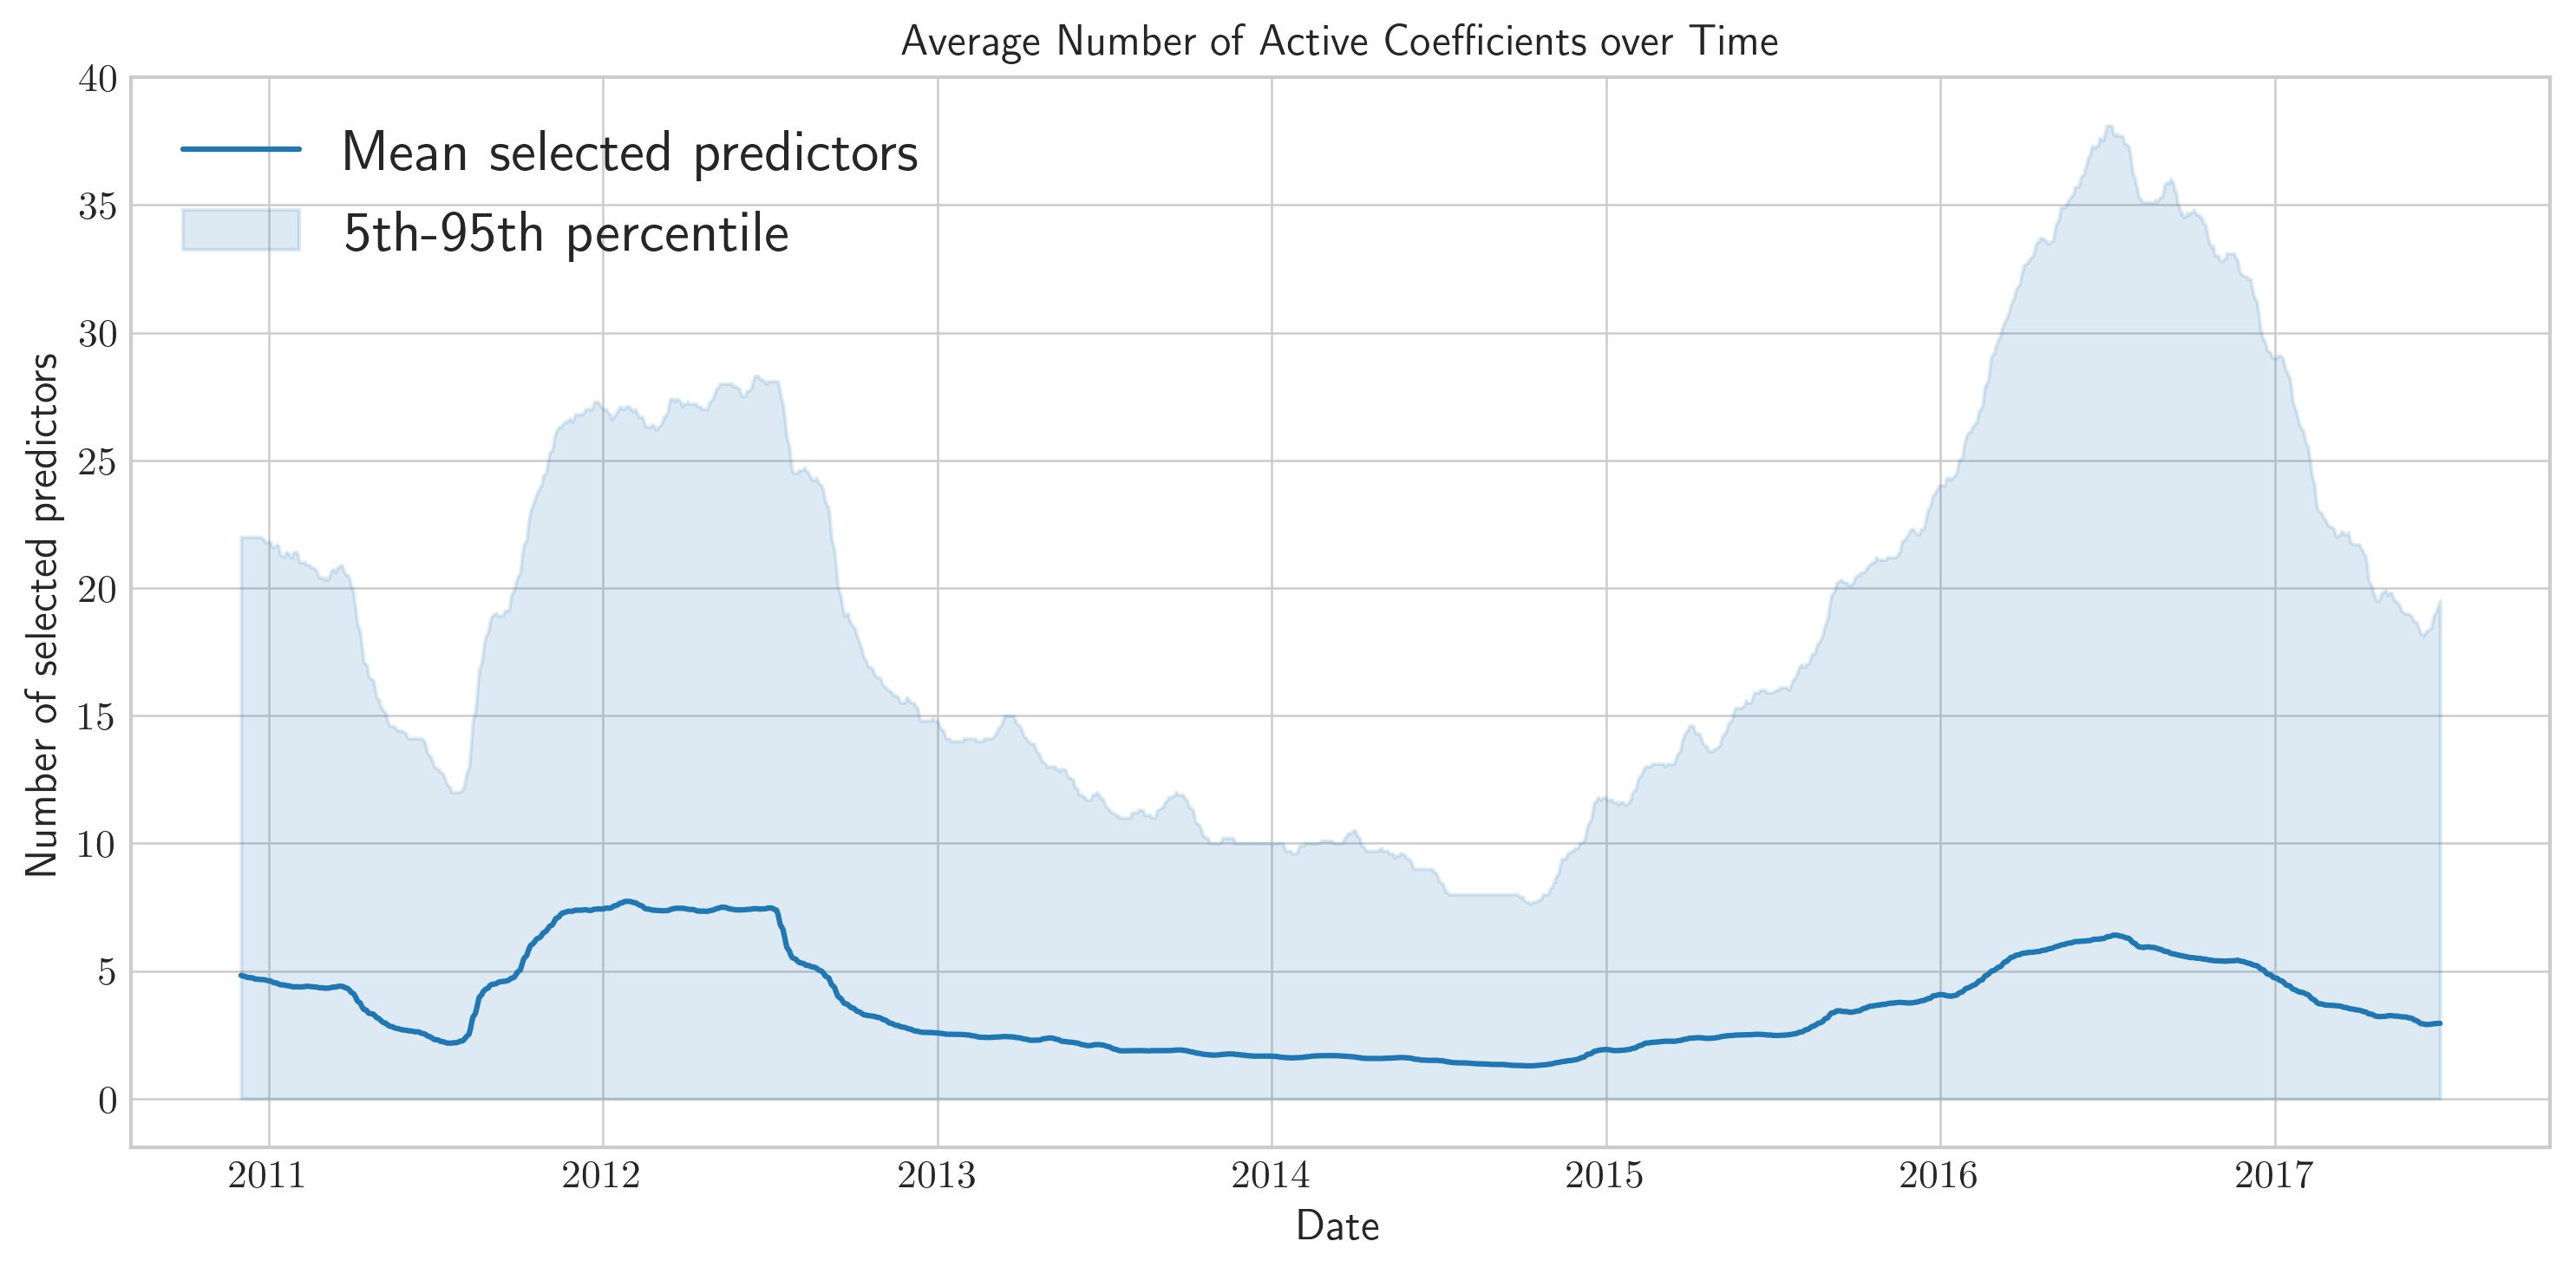
\includegraphics[width=0.7\textwidth]{active_coefficients_over_time.png}
    \caption{Average Number of Active Coefficients over Time}
    \label{fig:percent_active}
\end{figure}


We next examine \emph{which} features the LASSO selects.
The model makes a sharp prediction: because topic-attention innovations are globally standardised before entering the rolling window, there is no mechanical reason for any particular topic to be selected more frequently than another.
Selection probabilities should therefore be governed entirely by each topic’s statistical relationship with returns, producing an approximately uniform distribution across features.
To test this, we estimate the full beta tensor across all stocks and calculate the mean selection rate for each of the 190 features, defined as the proportion of stock-window observations in which the LASSO identifies a non-zero coefficient.

Figure~\ref{fig:topic_selection_freq} ranks the 190 candidate features by their mean selection rate.
While the distribution exhibits mild concentration (Gini coefficient = 0.18), it is not degenerate.
Every feature is selected at least once, and the most frequently selected feature (``Announce plan'', a news topic signaling corporate announcements) is selected $3.1\times$ above the uniform null rate.
The 10 macro time-series (highlighted in black) are selected at a rate only marginally higher than the 180 news topics on average ($1.1\times$), suggesting that no structural advantage accrues to macro series over news-topic signals.
The top two features are ``Announce plan'' and ``Financial reports'', both news topics signalling corporate activity and earnings news. The VIX, the most selected macro series, enters at rank 12.
Importantly, we find no evidence of the extreme concentration that would arise if a small subset of features mechanically dominated the selection process.
These results are consistent with selection being driven by statistical heterogeneity in return-predictive content rather than structural bias toward specific categories.

\begin{figure}[h]
    \centering
    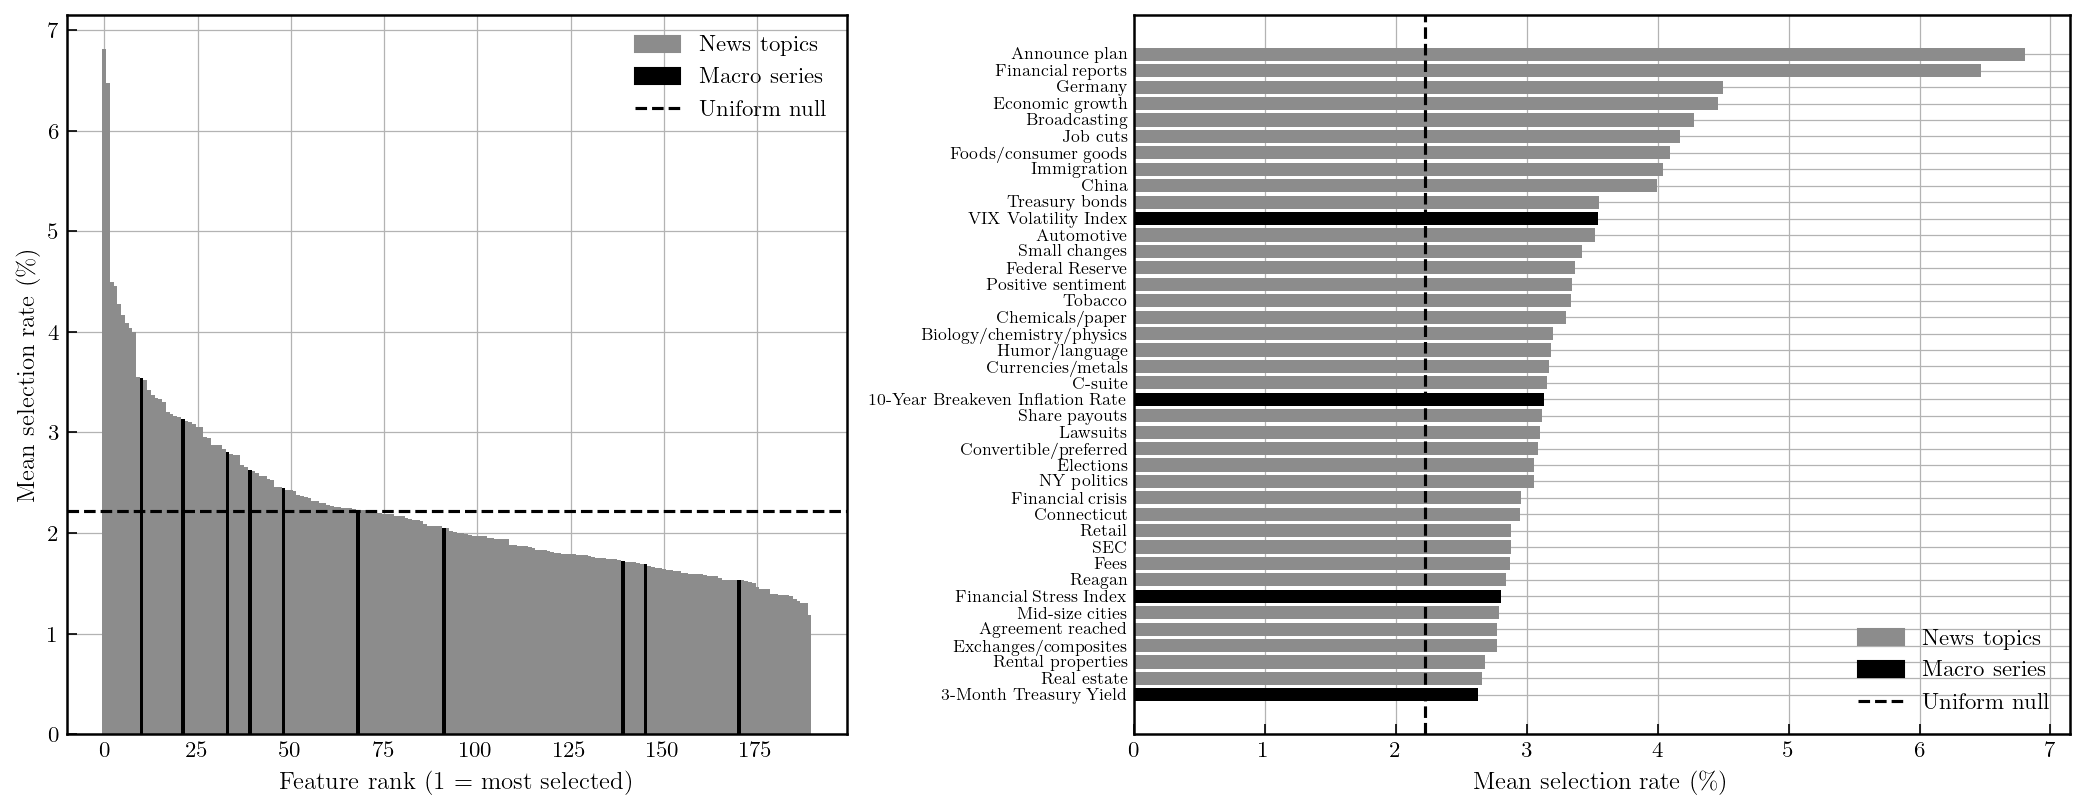
\includegraphics[width=\textwidth]{selection_frequency.png}
    \caption{LASSO Selection Frequency Across Features}
    \label{fig:topic_selection_freq}
    \begin{minipage}{\textwidth}
    \footnotesize
    \textit{Note:} Each bar represents the mean selection rate for a specific feature, defined as the proportion of stock-window observations with a non-zero LASSO coefficient across the 1,296 estimation stocks. Features are ordered by selection frequency. Red and blue bars distinguish the 10 macro time-series from the 180 news topics, respectively. The horizontal dashed line indicates the uniform null rate (total selections divided by 190). The left panel displays the full set of 190 features, while the right panel highlights the top 40 most frequently selected features.
    \end{minipage}
\end{figure}

\paragraph{Cross-Sectional Selection Intensity.}

Figure~\ref{fig:topic_selection_by_stock} characterizes the cross-sectional dimension of selection sparsity.
For each of the 1,296 stocks in our sample, we compute the average number of features selected per rolling window and plot the resulting distribution.
The distribution is markedly right-skewed and exhibits a significant mass at zero.
Consistent with our previous analysis, approximately 40\% of stocks average near zero selected features per window, reflecting the stringency of the global penalty for low-volatility assets.
Sectoral analysis reveals that Energy \& Mining stocks exhibit the highest selection intensity, likely driven by the persistent statistical signals of oil-market dynamics and higher baseline variance.
Conversely, stocks of financial firms display the lowest selection intensity.
Taken together with Figure~\ref{fig:topic_selection_freq}, these results establish that sparsity is a structural feature of the data in two dimensions: agents typically select only a parsimonious subset of available features for any individual stock (cross-feature sparsity), and the degree of this selection varies meaningfully across the investment universe (cross-sectional sparsity).

\begin{figure}[h]
    \centering
    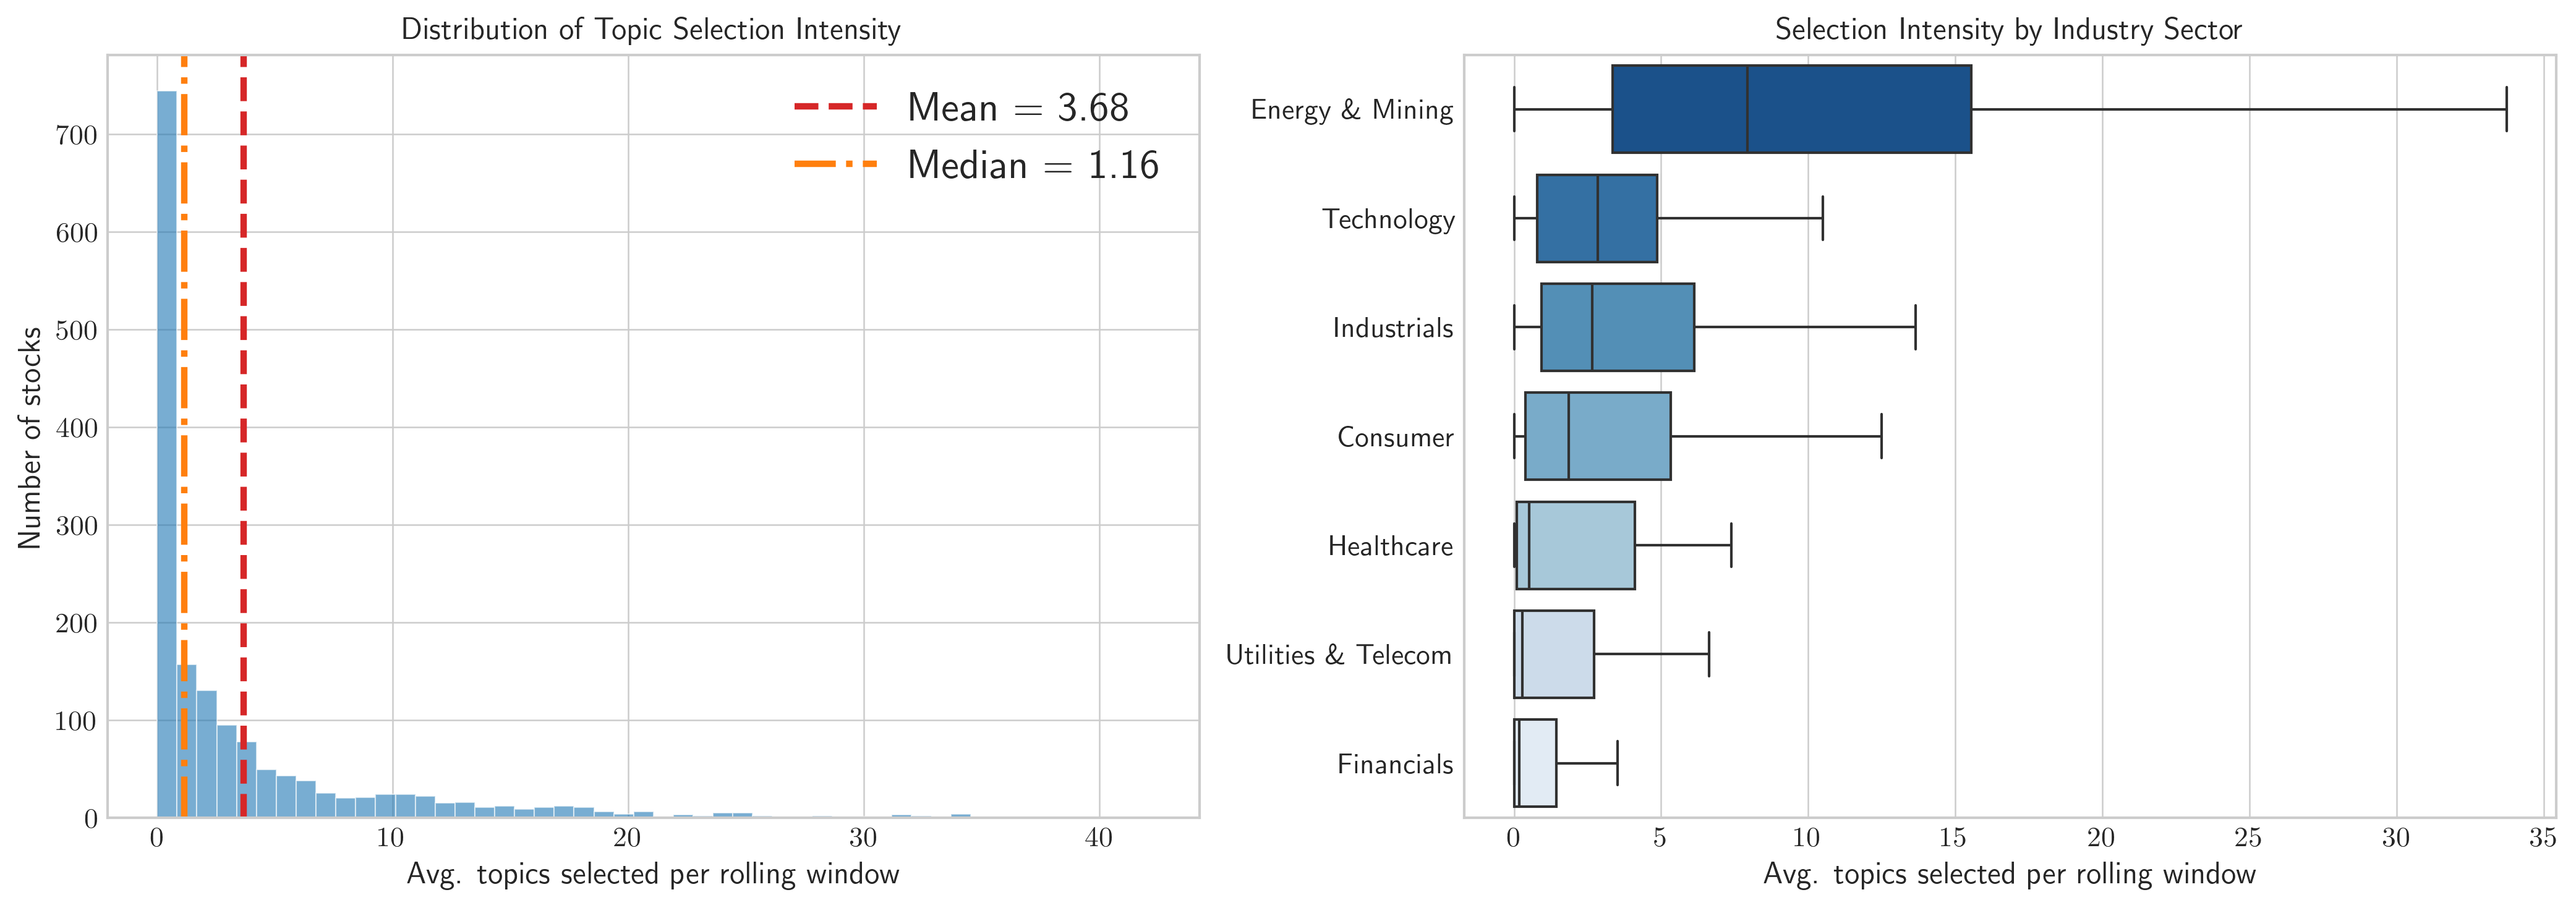
\includegraphics[width=\textwidth]{selection_intensity.png}
    \caption{LASSO Selection Intensity Across Stocks}
    \label{fig:topic_selection_by_stock}
    \begin{minipage}{\textwidth}
    \footnotesize
    \textit{Note:} Left panel: Histogram of the average number of features selected per rolling window across the 1{,}296 estimation stocks.
    Dashed red line is the cross-sectional mean; dash-dot orange line is the median.
    Right panel: Box plots of the same quantity by broad industry sector.
    \end{minipage}
\end{figure}

\paragraph{Time-series variation in selection intensity.}

Figure~\ref{fig:selection_rate_time} plots the cross-sectional mean, interquartile range, and p10--p90 band of the number of features selected per stock per rolling window, alongside the aggregate selection rate, over the full 2011--2017 sample.
Selection intensity exhibits significant temporal variation over the sample period.
The aggregate selection rate reaches its peak in January 2012 (4\%), coinciding with the height of the European sovereign debt crisis when macroeconomic news was highly informative for cross-sectional returns.
Conversely, the rate falls to a trough of 0.5\% in October 2014, reflecting a period of exceptional calm in U.S. equity markets.
This substantial range of variation confirms that perceived predictability is episodic, characterized by identifiable windows of signal detection interspersed with extended periods where few features clear the LASSO threshold.
Systemic events like the S\&P credit downgrade (August 2011), the ``taper tantrum'' (May 2013), the Chinese market turbulence (August 2015), the Brexit referendum, and the 2016 U.S. election—are all associated with visible surges in selection intensity.
These patterns are consistent with the view that macroeconomic uncertainty drives temporary increases in perceived return predictability.
The $p10$--$p90$ interval reveals that cross-sectional heterogeneity remains substantial at every point in time.
Even during peak episodes, many stocks select no feature, while a small subset selects multiple predictors simultaneously.
This persistent dispersion suggests that systematic episodes of predictability are not purely aggregate phenomena but are partly stock-specific, reflecting the subset of firms whose rolling-window estimates happen to exceed the selection threshold at a given date.

\begin{figure}[h]
    \centering
    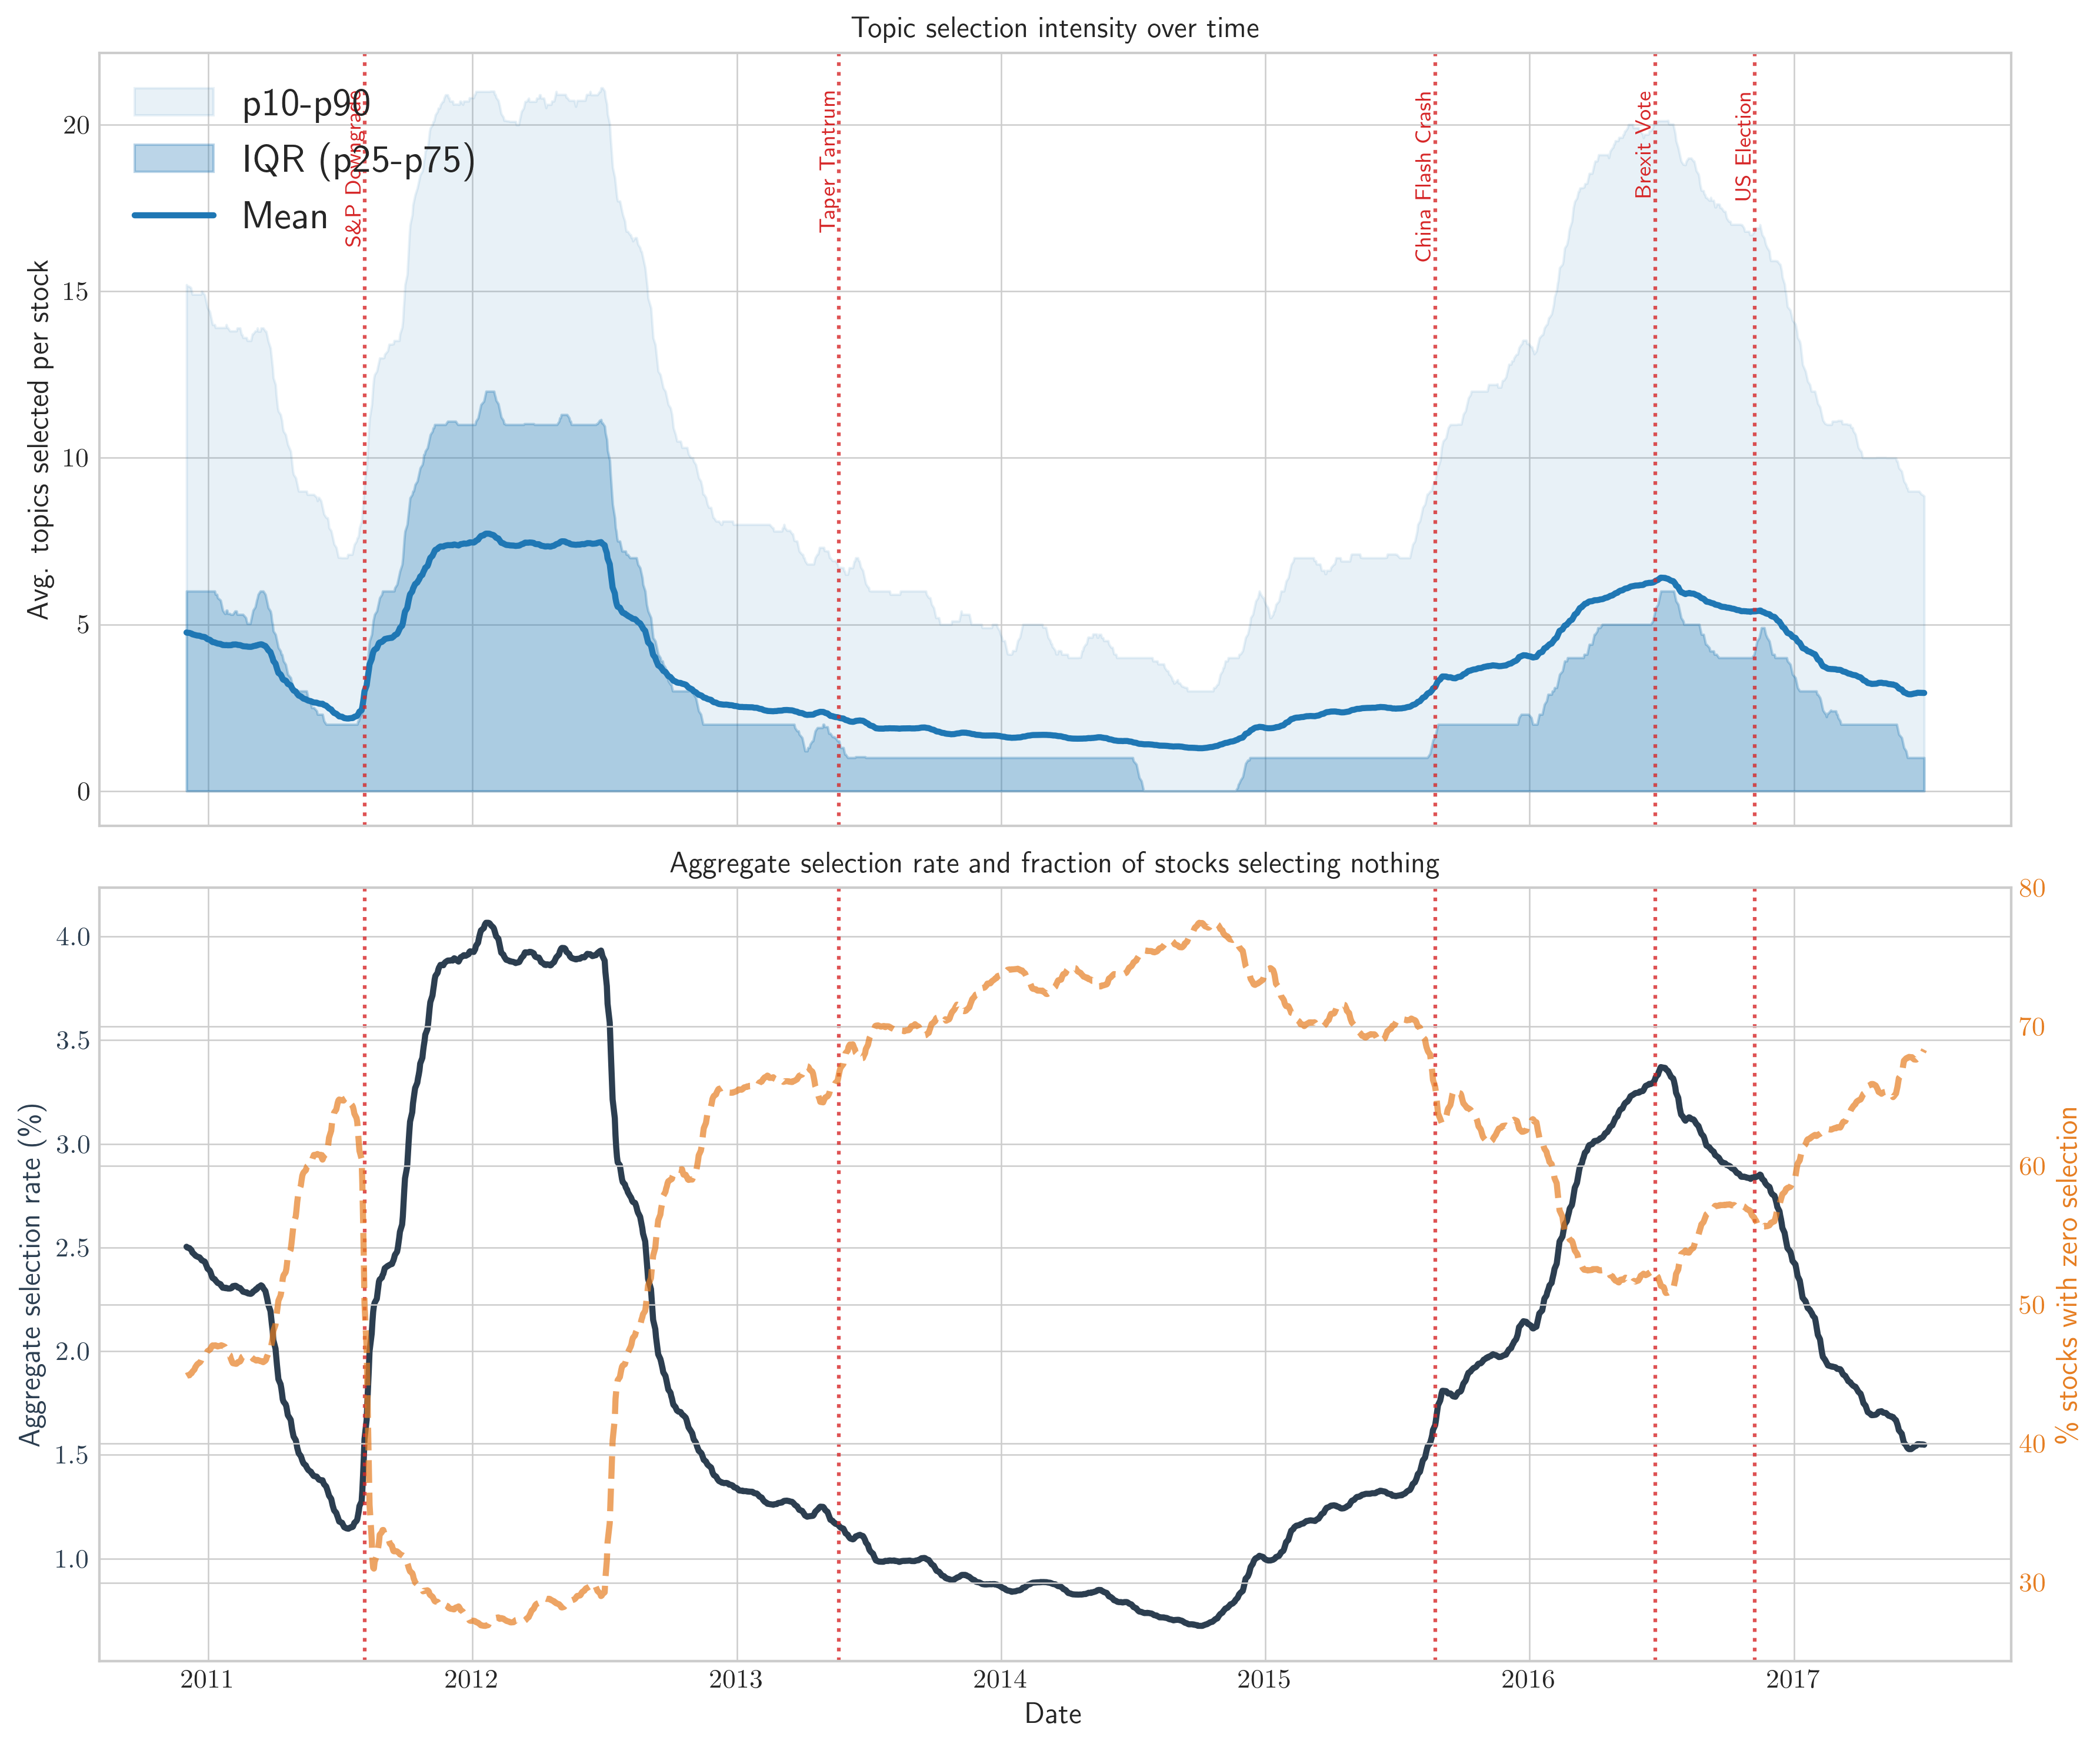
\includegraphics[width=\textwidth]{selection_intensity_over_time.png}
    \caption{Topic Selection Intensity Over Time}
    \label{fig:selection_rate_time}
    \begin{minipage}{\textwidth}
    \footnotesize
    \textit{Note:} \textbf{Top panel}: Cross-sectional distribution of the number of features selected per stock per rolling window (10-day centred moving average).
    Dark band = IQR (p25--p75); light band = p10--p90; line = cross-sectional mean.
    \textbf{Bottom panel}: Aggregate selection rate (fraction of all stock-feature pairs with a non-zero LASSO coefficient, left axis) and fraction of stocks selecting zero features (right axis, dashed orange).
    Red dashed vertical lines mark selected macro events within the sample period.
    \end{minipage}
\end{figure}

\paragraph{What drives time-series variation in selection intensity?}
The time-series variation in selection rates is informative about the mechanism.
Under the CMCE equilibrium with constant idiosyncratic volatility $\sigma_u$, the
expected selection rate is flat: any systematic co-movement with observable volatility
measures must stem from sources outside the baseline model.
We decompose this variation along two dimensions.

\emph{Regression evidence.}
We regress the aggregate selection rate $\bar{s}_t$ on two volatility proxies: (i)~the
cross-sectional standard deviation of daily returns $\sigma_{r,t}$, measuring the
overall informational environment, and (ii)~the average absolute topic activity
$\sigma_{x,t}$, measuring how much the predictors are fluctuating.
The sign predictions follow directly from the LASSO mechanism: higher return volatility
inflates the apparent magnitude of sample OLS coefficients and thus raises the
probability of clearing the threshold ($+$), while higher predictor volatility deflates
standardised coefficients and lowers it ($-$).
Estimating the regression with Newey--West standard errors (20 lags), we find
$R^2 = 0.12$, with $\hat\beta_{\sigma_r} = +0.188$ ($t = 3.22$, $p < 0.01$) and
$\hat\beta_{\sigma_x} = -0.170$ ($t = -3.07$, $p < 0.01$)---both significant with
the predicted sign.

\emph{Oracle simulation.}
To assess how much of the residual variation is consistent with the model's finite-sample
mechanism, we run an oracle exercise: we replace actual returns with i.i.d.\
$\mathcal{N}(0, \hat\sigma_{u,i}^2)$ draws for 150 stocks and re-run the same rolling
LASSO at each stock's estimated $\lambda_i$ with the common fixed window $s=252$.
Under i.i.d.\ noise with constant variance, the model implies a selection rate that is
essentially flat across time.
Indeed, the simulated aggregate selection rate has a standard deviation 19$\times$ smaller
than the actual one, and the Spearman correlation between the two series is $\rho = 0.02$
($p = 0.31$).
This confirms that the bulk of the observed time variation is \emph{extra-model}: it
cannot be generated by i.i.d.\ noise alone, even at the empirically calibrated
$\sigma_{u,i}$.
Figure~\ref{fig:selection_rate_decomposition} reports the actual vs.\ simulated selection
rates alongside the regression decomposition.

\begin{figure}[H]
    \centering
    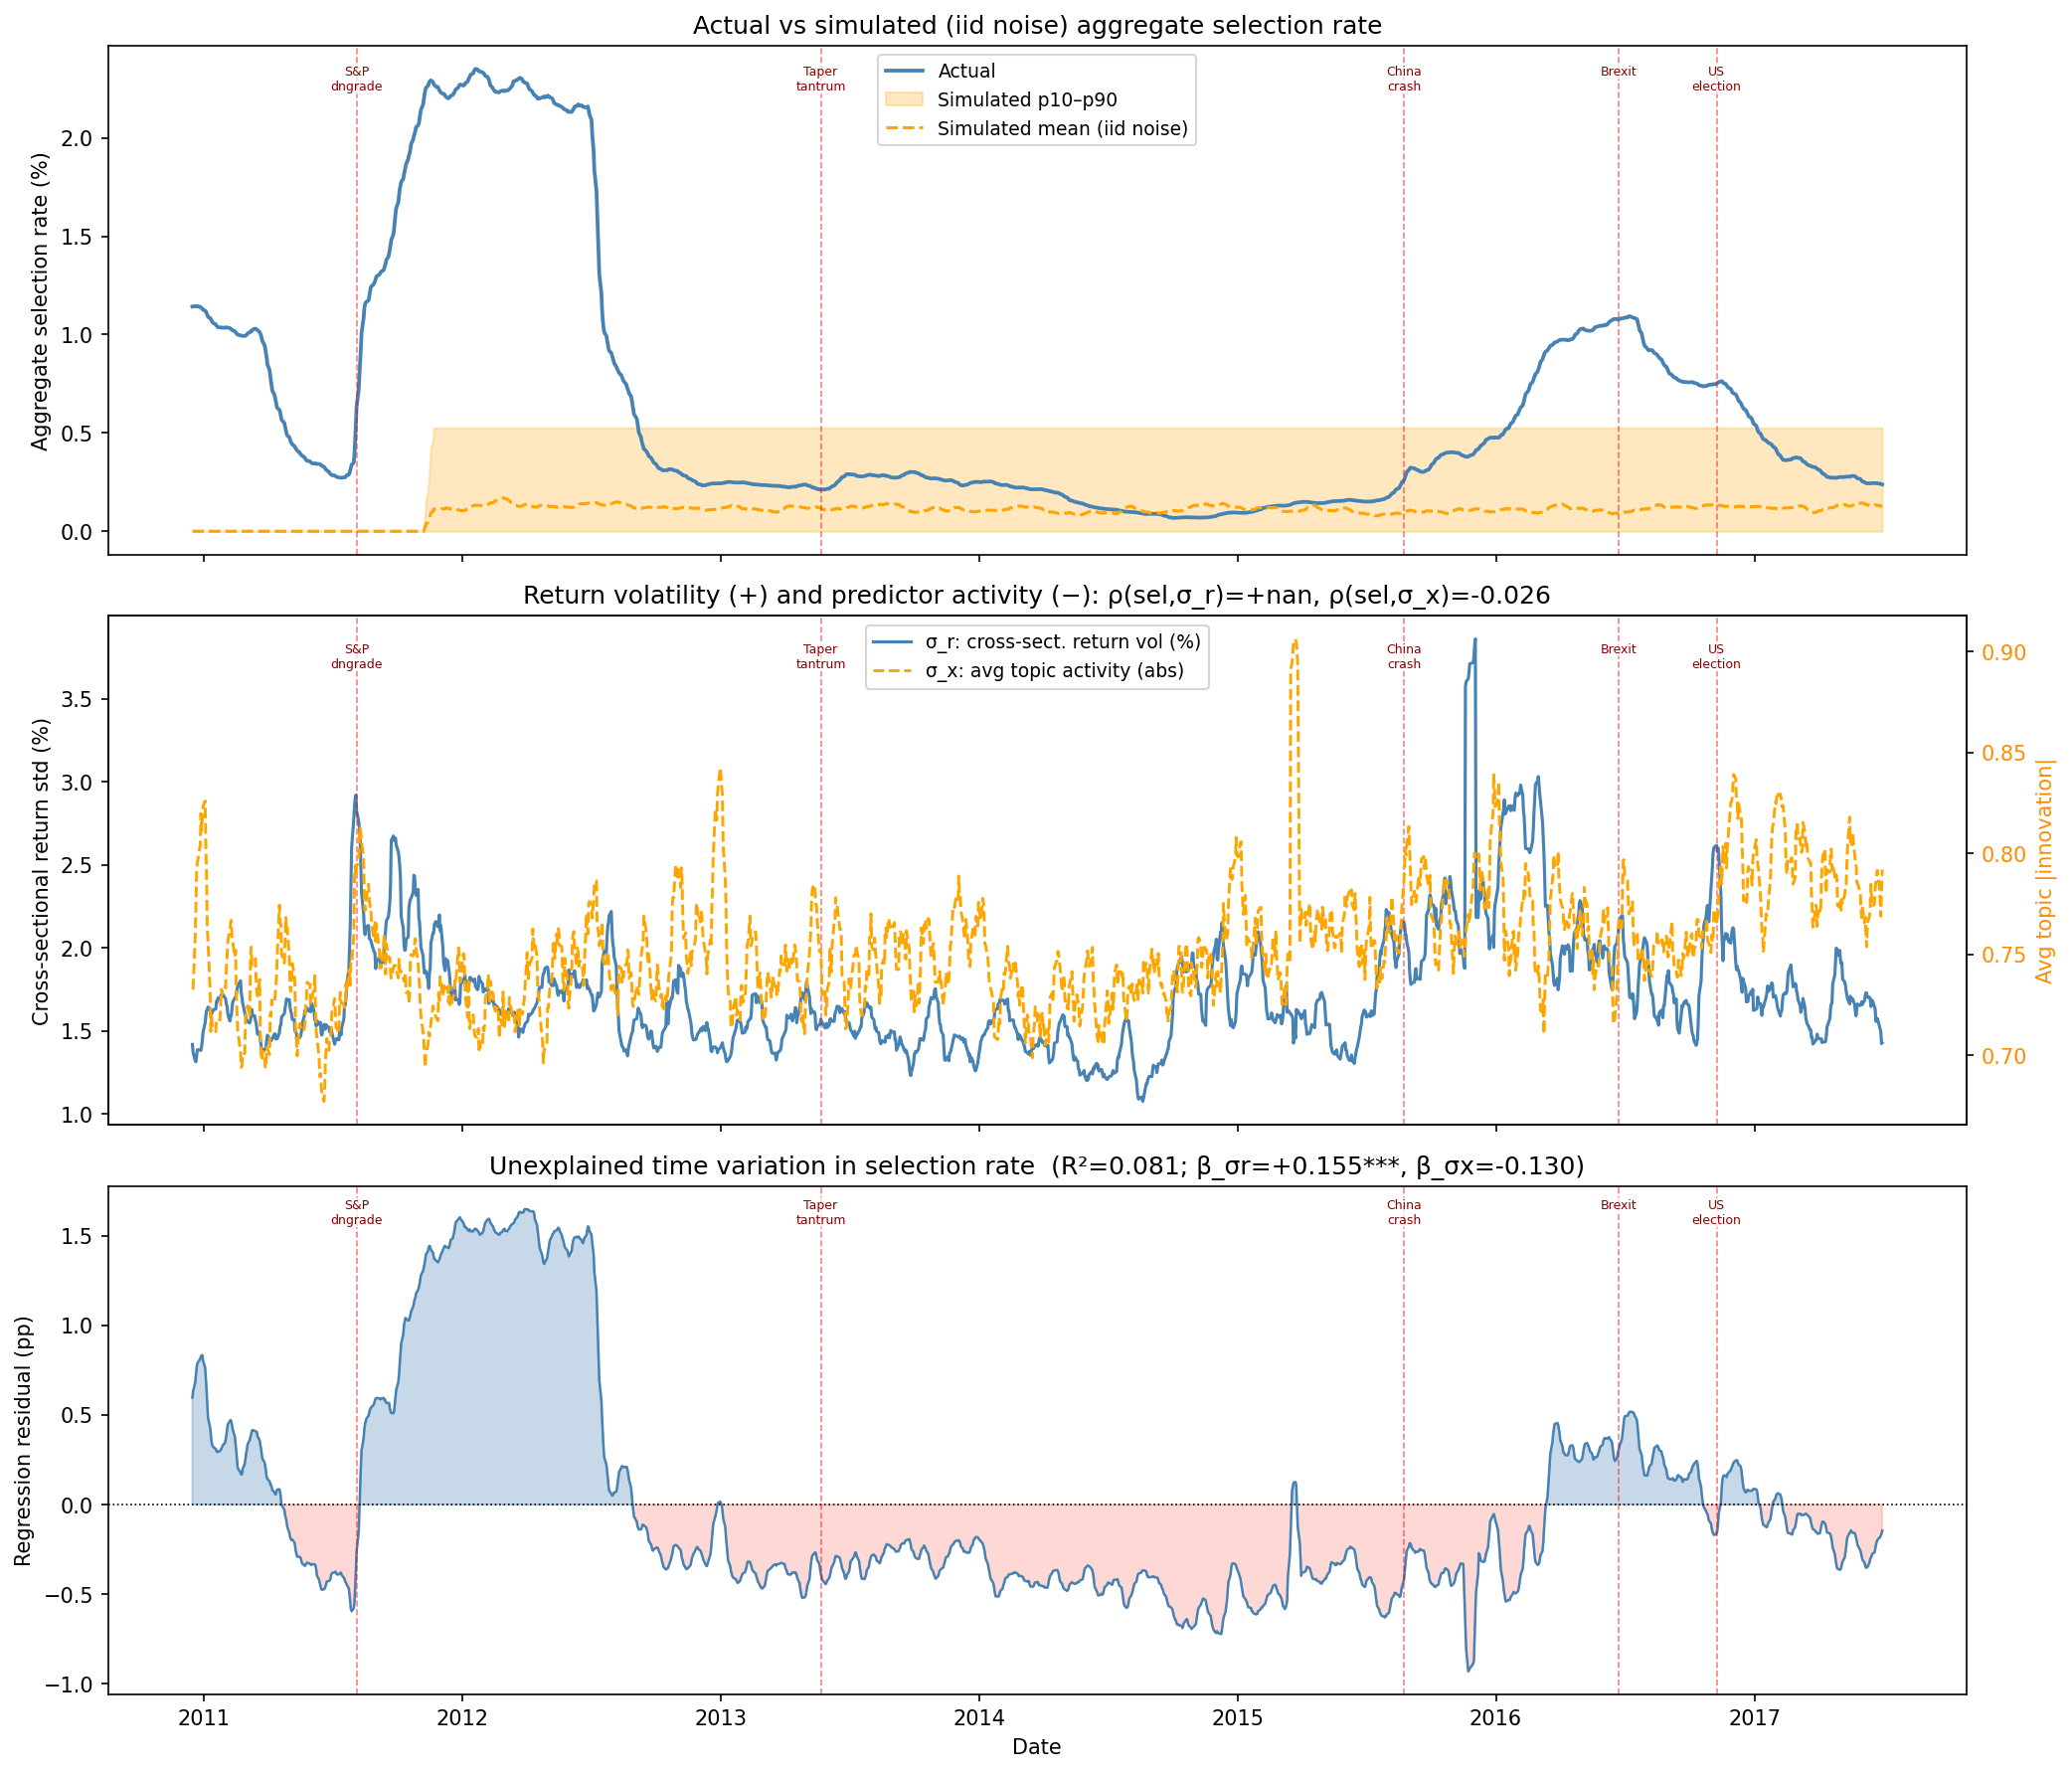
\includegraphics[width=\textwidth]{selection_rate_decomposition.png}
    \caption{Decomposition of Time-Series Variation in Aggregate Selection Rate}
    \label{fig:selection_rate_decomposition}
    \begin{minipage}{\textwidth}
    \footnotesize
    \textit{Note:} \textbf{Top panel}: actual aggregate selection rate (blue) against
    the i.i.d.\ oracle simulation (orange dashed = mean; shaded = p10--p90 across 150
    stocks). \textbf{Middle panel}: cross-sectional return volatility $\sigma_{r,t}$
    (blue, left axis) and average absolute topic activity $\sigma_{x,t}$ (orange, right
    axis). \textbf{Bottom panel}: OLS residual from the regression
    $\bar{s}_t = a + b_1\sigma_{r,t} + b_2\sigma_{x,t} + \varepsilon_t$
    with Newey--West standard errors (20 lags); $R^2 = 0.12$.
    Red dashed lines mark selected macro events.
    \end{minipage}
\end{figure}

\paragraph{GARCH volatility as the missing ingredient.}
The 19-fold gap between actual and i.i.d.-oracle selection-rate variance motivates
extending the noise term to a GARCH structure.
Economically, the idiosyncratic component $u_{i,t}$ in the ALM---the gap between
realised returns and the agents' belief-driven demand signal---represents
\emph{unspanned fundamental shocks}: earnings surprises, idiosyncratic supply-demand
imbalances, and liquidity effects that the PLM's topic vocabulary cannot capture.
There is a natural reason for this residual to exhibit volatility clustering: fundamental
uncertainty is itself state-dependent.
During episodes of macro stress---credit crunches, monetary policy surprises, geopolitical
shocks---both the magnitude and the cross-sectional correlation of these fundamental
shocks expand.
This is captured by a factor structure
$u_{i,t} = \sigma_{m,t}\eta_t^{(m)} + \tilde\sigma_i\eta_{i,t}^{(i)}$, where $\sigma_{m,t}$
follows a GARCH$(1,1)$ process fitted to VW market returns.
When $\sigma_{m,t}$ spikes, all stocks simultaneously face larger noise relative to their
rolling-window OLS estimates, pushing more topic coefficients above the LASSO threshold
purely by chance---generating the synchronised, aggregate selection spikes we observe.

To quantify this, we simulate 150 stocks replacing i.i.d.\ noise with GARCH noise calibrated
to each stock's market beta and idiosyncratic volatility, and re-run the same rolling LASSO.
The GARCH simulation reduces the actual/simulated standard deviation ratio from 19$\times$
(i.i.d.) to \textbf{1.32$\times$}, and the Spearman correlation between actual and simulated
aggregate selection rates rises from $\rho = 0.02$ (i.i.d., $p = 0.31$) to
$\rho = +0.38$ (GARCH, $p < 0.0001$): the timing of selection spikes is largely recovered.
Replacing the raw cross-sectional return volatility with the GARCH conditional volatility
$\sigma_{m,t}$ in the regression further raises $R^2$ from $0.12$ to $0.18$
($\hat\beta_{\sigma_m} = +0.242$, $t = 3.83$; $\hat\beta_{\sigma_x} = -0.132$, $t = -2.47$).
Figure~\ref{fig:garch_oracle} shows the comparison.

\begin{figure}[H]
    \centering
    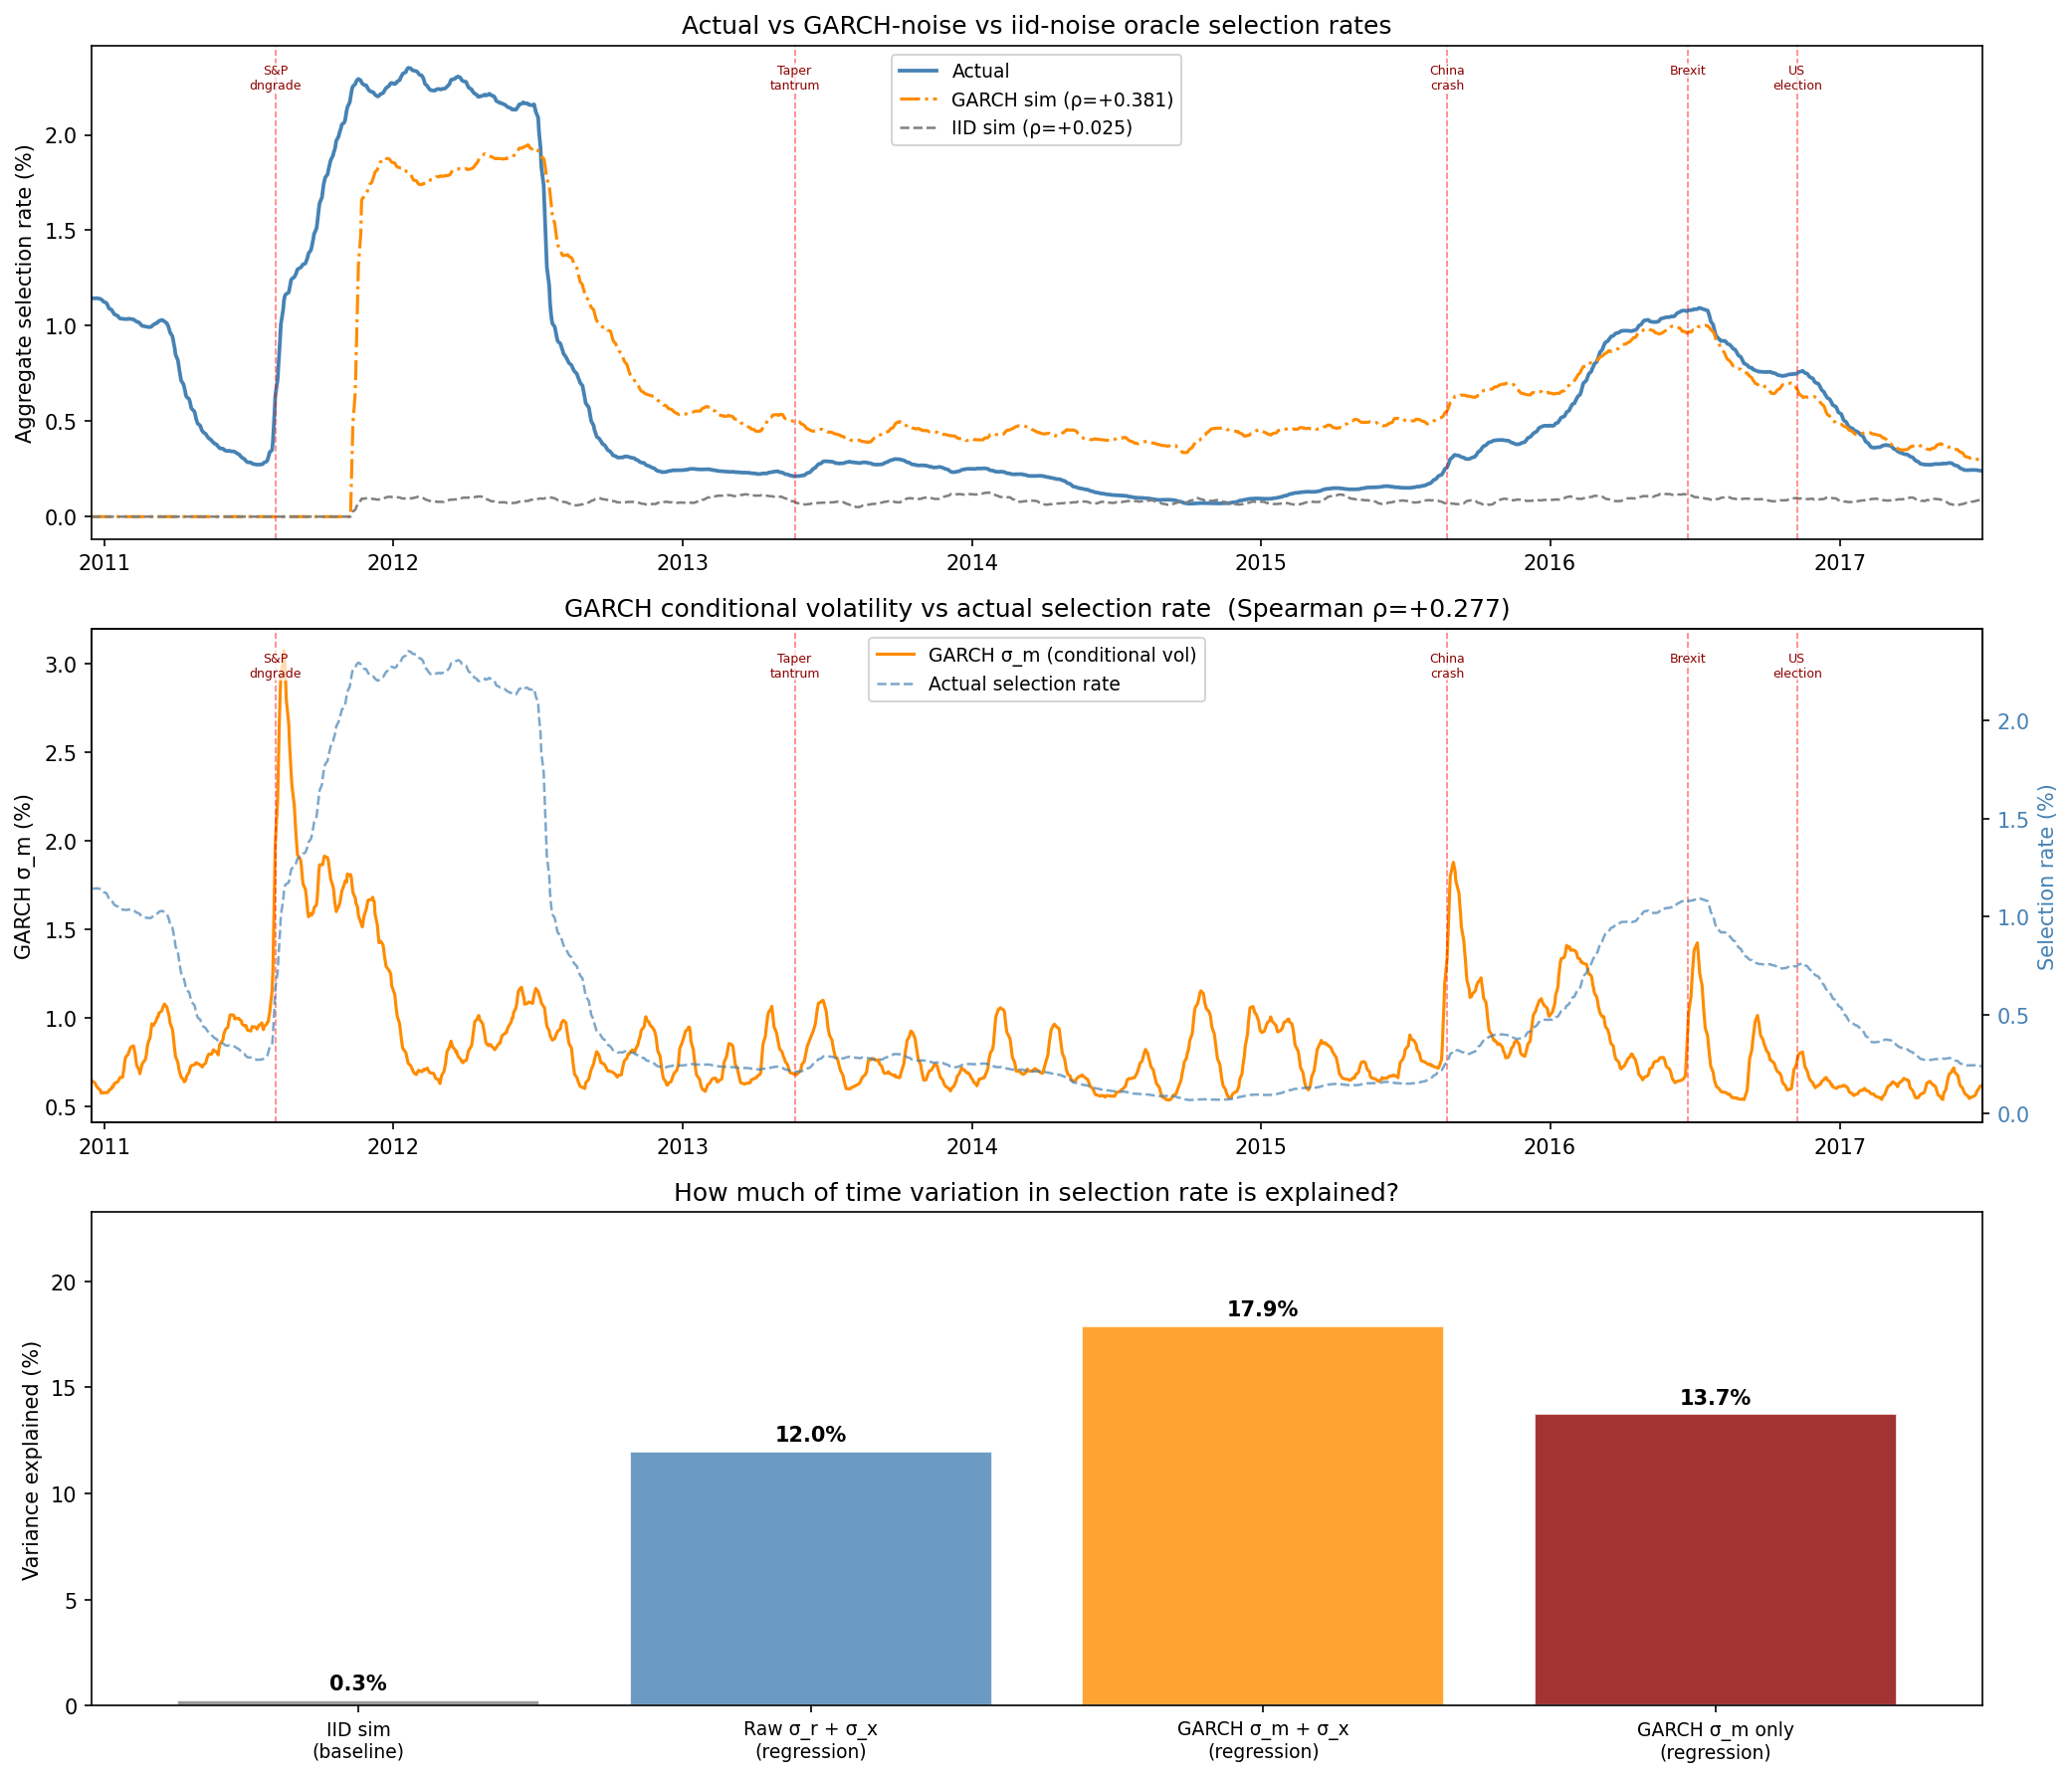
\includegraphics[width=\textwidth]{garch_selection_oracle.png}
    \caption{GARCH Oracle: Actual vs.\ Simulated Selection Rates}
    \label{fig:garch_oracle}
    \begin{minipage}{\textwidth}
    \footnotesize
    \textit{Note:} \textbf{Top panel}: actual aggregate selection rate (blue) against
    the GARCH oracle (orange, mean $\pm$ p10--p90 band) and the i.i.d.\ oracle (grey,
    mean).
    \textbf{Middle panel}: GARCH conditional volatility $\hat\sigma_{m,t}$ from a
    GARCH$(1,1)$ fitted to daily VW market returns (orange), overlaid with the actual
    selection rate (blue dashed).
    \textbf{Bottom panel}: fraction of actual selection-rate variance explained by four
    specifications: i.i.d.\ oracle variance ratio, regression on raw $\sigma_r + \sigma_x$
    ($R^2 = 0.12$), regression on GARCH $\sigma_m + \sigma_x$ ($R^2 = 0.18$), and
    GARCH $\sigma_m$ alone ($R^2 = 0.14$).
    The estimated GARCH persistence parameter is $\hat\alpha + \hat\beta = 0.96$.
    \end{minipage}
\end{figure}

Taken together, these results imply that the dominant driver of episodic selection
spikes is time-varying fundamental uncertainty with a common factor structure---not
genuine predictability.
The CMCE mechanism translates fluctuations in $\sigma_{m,t}$ into apparent topic
selections: when the market enters a high-volatility regime, the same LASSO procedure
that would be flat under constant noise instead registers a broad, synchronised burst
of perceived predictability.
As volatility subsides, the rolling-window coefficients revert and selections disappear,
exactly as the CMCE equilibrium predicts.
This finding is also consistent with the narrative economics view of \citet{Shiller2017}:
periods of heightened fundamental uncertainty are precisely when new narratives spread
most rapidly, as agents search for explanations and update their PLMs more aggressively.
In our framework, this search is disciplined by the LASSO threshold---but under a
GARCH volatility regime, that threshold is more frequently cleared by chance, producing
the episodic, crisis-coincident predictability bursts documented in
Figure~\ref{fig:selection_rate_time}.

\paragraph{Persistence of topic selection.}

We investigate the temporal properties of selection episodes to determine whether a topic, once selected for a specific stock, remains active in subsequent rolling windows.
Figure~\ref{fig:topic_selection_persistence} characterizes this persistence across three complementary dimensions.
The \emph{run-length distribution} (top-left panel), pooled across 623,223 selection episodes, is markedly right-skewed.
While the median run length is only 4 windows (approximately one trading week), the 95th percentile reaches 78 windows, with a maximum observed length of 544.
This distribution suggests the coexistence of two distinct regimes: a majority of transient selections that are discarded as new data enter the window, and a minority of highly persistent episodes where the statistical signal is sufficiently robust to survive numerous updates.
The \emph{survival curve} (top-right panel) estimates the conditional probability $P(\text{selected at } t+k \mid \text{selected at } t)$ for lags up to 120 windows.
Persistence decays rapidly in the immediate term, with 74\% of events surviving to the next window and 41\% to the fifth—before the curve flattens considerably.
Notably, 18\% of episodes persist to lag 20 and 7\% survive to lag 60, representing roughly three months of trading.
This slow-decaying tail aligns with the CMCE mechanism, wherein a selected topic generates self-fulfilling predictability that sustains itself until the rolling-window estimate is sufficiently diluted by new observations.
The \emph{mean autocorrelation function} (bottom-left panel), averaged over 86,358 active stock-topic pairs, further substantiates this temporal dependence.
The first-order autocorrelation is 0.89 and exhibits a gradual decay ($\text{AC}(5) = 0.73$, $\text{AC}(20) = 0.46$), diverging significantly from the near-zero values expected under an i.i.d.\ selection process.
Finally, the bottom-right panel provides a representative heatmap of selection activity for the stock with the highest average selection rate.
Rather than a uniform or rotating pattern, the heatmap reveals that a concentrated set of features is selected repeatedly across non-overlapping windows.
These results suggest that certain topic--stock pairs represent genuinely recurring statistical relationships that market agents periodically rediscover.

\begin{figure}[h]
    \centering
    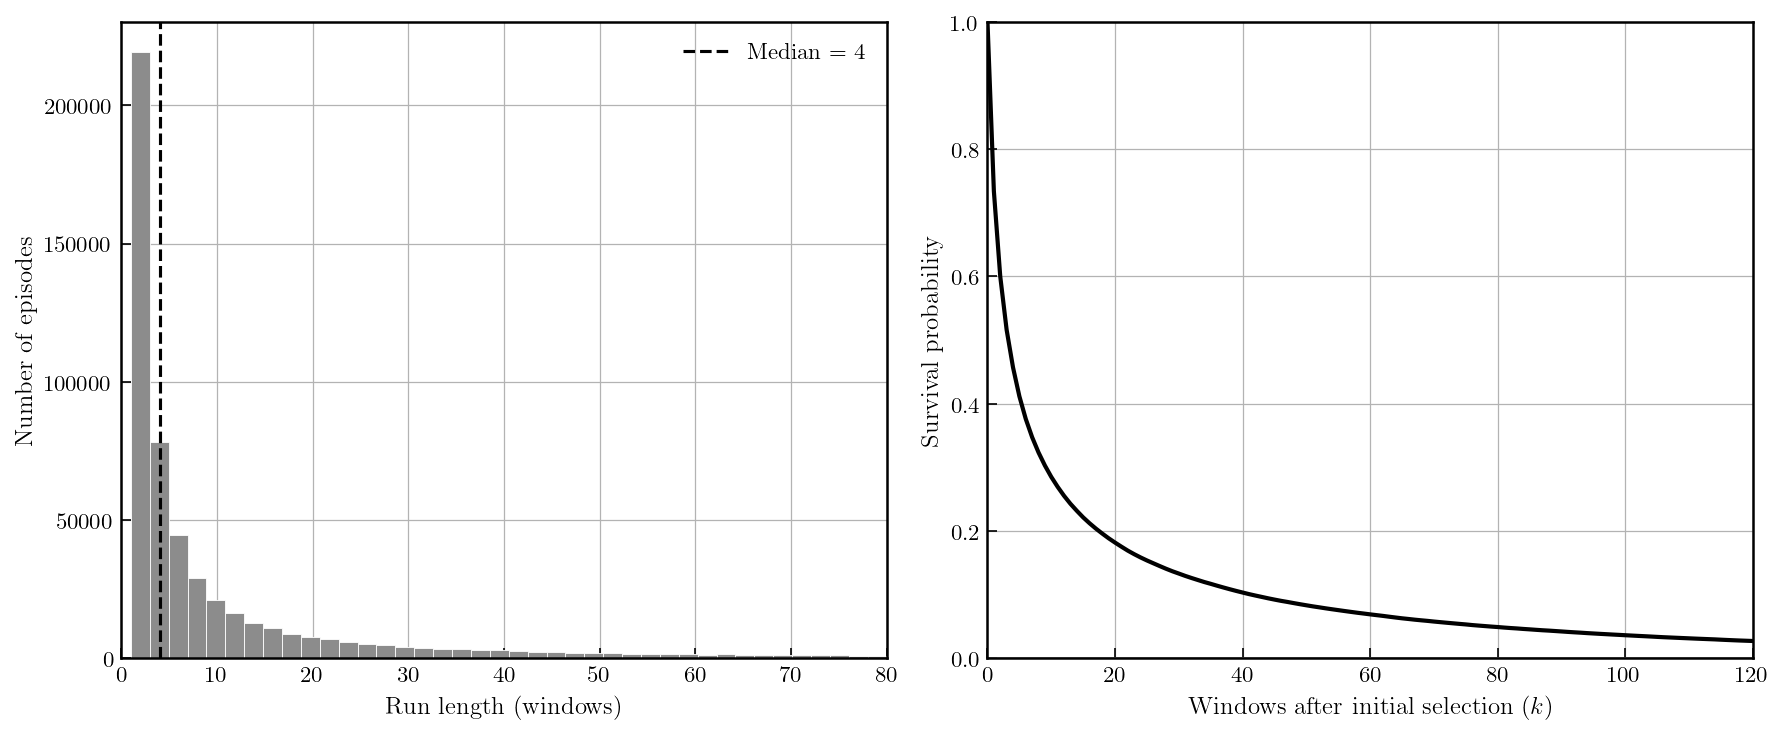
\includegraphics[width=\textwidth]{distribution_survival_autocorrelation.png}
    \caption{Persistence of Topic Selection Episodes}
    \label{fig:topic_selection_persistence}
    \begin{minipage}{\textwidth}
    \footnotesize
    \textit{Note:} All panels are based on 1,296 stocks, 190 features and 1,648 trading days. 
    \textbf{Top-left}: Histogram of run lengths (consecutive windows a topic remains selected), pooled across 623,223 episodes; truncated at 80 windows for readability. 
    \textbf{Top-right}: Survival curve $P(\text{selected at }t+k \mid \text{selected at }t)$ estimated for each onset event and averaged across all stock-topic pairs. 
    \textbf{Bottom-left}: Mean autocorrelation function of the binary selection indicator, averaged over 86,358 active stock-topic pairs (mean selection rate $\geq 0.5\%$). 
    \textbf{Bottom-right}: Heatmap of topic selection over time for the most actively selected stock (top 30 topics by total selection count; every 5th window plotted).
    \end{minipage}
\end{figure}

\paragraph{Narrative alignment.}

While our model posits that feature selection is driven purely by statistical properties, we investigate whether a non-statistical component also plays a role: do agents disproportionately select features that are ``narratively coherent'' with a firm's core business?
Because the penalty, $\lambda$, mechanically induces higher selection frequencies for highly volatile stocks, we use stock-level fixed effects to absorb these baseline differences.
Consequently, any residual variation in how often different features are selected for a given stock must reflect either the true statistical relationship between the topic and the stock's returns, or its narrative relevance.
To quantify this narrative relevance, we measure the linguistic overlap between the predictive topics and the firm's own self-description.
We extract the formal business description from each firm's annual 10-K report, specifically the section legally mandated by the SEC as ``Item 1: Business''.
For the 591 firms with available documents in the EDGAR database, we compute a TF-IDF vector of this text and compare it against the TF-IDF vector of key terms for each of the 180 news-topics.
The resulting cosine similarity, $\cos_{ij} \in [0,1]$, serves as our proxy for how closely topic $j$'s vocabulary aligns with firm $i$'s stated economic identity.
We estimate this relationship using the following panel regression:

\begin{equation}\label{eq:narrative_reg}
\bar{s}_{ij} = \alpha_i + \delta_j + \beta \cos_{ij} + \varepsilon_{ij},
\end{equation}

where $\bar{s}_{ij}$ is the mean LASSO selection rate for stock $i$ and feature $j$.
The inclusion of stock fixed effects, $\alpha_i$, absorbs firm-level differences in overall selection propensity, while feature fixed effects, $\delta_j$, account for the aggregate popularity of specific topics.
Thus, the coefficient $\beta$ isolates the precise within-firm, within-topic effect of narrative alignment.
Table~\ref{tab:narrative_alignment} reports the results.
Across 112,290 stock-topic observations, we find a statistically significant but economically modest effect. 
A one-standard-deviation increase in cosine similarity raises the residual selection rate by 0.00012 percentage points.
The overall Spearman rank correlation is also positive and highly significant.
Notably, as shown in Panel B, this narrative alignment is concentrated in the Consumer and Financial sectors, but is entirely absent or reversed in Technology and Healthcare.
We additionally test a between-firm hypothesis: are ``narratively central'' firms, meaning those whose business descriptions broadly overlap with the vocabulary of the entire feature set, more likely to have topics selected overall?
Using the average cosine similarity across all 180 topics as a proxy for a firm's narrative centrality, we find no significant correlation with its mean selection rate.
The most narratively central stocks, such as regional banks and utilities, naturally use broad financial terminology that overlaps with many topics, which rules out a mechanical link between a firm's language breadth and its overall selection frequency.
Ultimately, these findings suggest that while statistical relevance remains the primary driver of feature selection, a marginal narrative alignment effect persists in specific sectors.
Agents appear slightly more inclined to act on statistical signals when those signals resonate with their prior understanding of a firm's established economic identity, an observation consistent with the narrative economics framework of \citet{Shiller2017}.

\begin{table}[H]
\centering
\caption{Narrative Alignment: 10-K Similarity and LASSO Selection Rates}
\label{tab:narrative_alignment}
\begin{tabularx}{\textwidth}{@{}>{\small}X r r r r r@{}}
\toprule
 & $N_{\text{stocks}}$ & $N_{\text{obs}}$ & Spearman $\rho$ & Panel FE $\hat\beta$ & $t$-stat \\
\midrule
\multicolumn{6}{l}{\textit{Panel A: All sectors pooled}} \\[2pt]
Overall   & 591 & 112{,}290 & $+0.026^{***}$ & $0.0088$ & $2.02^{**}$ \\[6pt]
\multicolumn{6}{l}{\textit{Panel B: By sector}} \\[2pt]
Energy \& Mining      & 36  & 6{,}840  & $+0.021^{*}$   & $0.0074$ & $0.39$ \\
Financials            & 137 & 26{,}030 & $+0.036^{***}$ & $0.0147$ & $1.85^{*}$ \\
Technology            & 25  & 4{,}750  & $-0.002$        & $-0.0302$ & $-1.06$ \\
Healthcare            & 13  & 2{,}470  & $-0.022$        & $0.0427$ & $0.99$ \\
Consumer              & 71  & 13{,}490 & $+0.014$        & $0.0652$ & $5.19^{***}$ \\
Industrials           & 101 & 19{,}190 & $+0.022^{***}$ & $-0.0157$ & $-1.38$ \\
Utilities \& Telecom  & 35  & 6{,}650  & $+0.085^{***}$ & $0.0158$ & $0.79$ \\[6pt]
\multicolumn{6}{l}{\textit{Panel C: Between-stock narrative centrality}} \\[2pt]
Mean sim.\ vs.\ mean sel.\ rate & 591 & --- & $+0.049$ & --- & --- \\
\bottomrule
\end{tabularx}
\medskip
\begin{minipage}{\textwidth}
\footnotesize
\textit{Note:} $\bar{s}_{ij}$ is the mean LASSO selection rate for stock $i$ and feature $j$ across all rolling windows.
Cosine similarity $\cos_{ij}$ is computed between TF-IDF vectors of each firm's 10-K Business Description (Item~1) and the key-term string of each WSJ topic feature.
Panel FE $\hat\beta$ is from OLS on the within-transformed data with stock and topic fixed effects.
Panel~C reports the Spearman correlation between each firm's average cosine similarity across all features (``narrative centrality'') and its average selection rate.
Significance is denoted as $^{*}p<0.10$, $^{**}p<0.05$, $^{***}p<0.01$.
\end{minipage}
\end{table}

\subsection{Robustness: Volatility-Scaled Penalty}

The baseline specification uses a single global $\lambda$ across all stocks.
Because the topic features $X_t$ are standardised within each rolling window but the
return $r_{i,t}$ is not, the effective penalisation relative to the signal-to-noise
ratio varies with stock volatility.
Specifically, the LASSO soft-thresholding condition implies that a predictor is selected
only if its within-window OLS coefficient exceeds $\lambda$ in absolute value.
For a low-volatility stock (small $\sigma_i$), returns fluctuate less, so OLS coefficients
are smaller in magnitude and $\lambda$ is proportionally more restrictive, which explains
why $\approx 40\%$ of stocks have zero LASSO selection under the global $\lambda$.
A natural robustness check replaces $\lambda$ with a per-stock volatility-scaled penalty:
\begin{equation}\label{eq:volscaled_lambda}
\lambda_i = \lambda \times \frac{\sigma_i}{\bar\sigma},
\end{equation}
where $\sigma_i = \mathrm{std}(r_{i,\cdot})$ is the full-sample standard deviation of stock $i$'s
log returns and $\bar\sigma = 0.0175$ is the cross-sectional median.
This normalisation restores a uniform effective penalty relative to each stock's return scale.
The window $s$ is kept at the baseline value, and we continue to use one lag of topic innovations; no additional hyperparameter
optimisation is performed for this specification.
Table~\ref{tab:comparison} reports a side-by-side comparison of the two specifications on the
same 1,296 estimation stocks.
 
\begin{table}[H]
\centering
\caption{Baseline vs.\ Volatility-Scaled Penalty: Estimation Results}
\label{tab:comparison}
\begin{tabularx}{\textwidth}{@{}>{\small}X cc cc@{}}
\toprule
 & \multicolumn{2}{c}{Baseline ($\lambda = 3.224\!\times\!10^{-3}$)}
 & \multicolumn{2}{c}{Vol-scaled ($\lambda_i = \lambda\sigma_i/\bar\sigma$)} \\
\cmidrule(lr){2-3}\cmidrule(lr){4-5}
 & mean & median & mean & median \\
\midrule
\multicolumn{5}{l}{\textit{Stage 1 — all estimation stocks ($N=1{,}296$)}} \\[2pt]
In-sample $R^2$    & 0.0249 & 0.0071 & 0.0081 & 0.0072 \\
OOS $R^2$          & $-$0.0116 & $-$0.0036 & $-$0.0048 & $-$0.0036 \\
Selection rate     & 0.0222 & 0.0071 & 0.0064 & 0.0061 \\
\% zero selection  & \multicolumn{2}{c}{40.5\%}  & \multicolumn{2}{c}{3.2\%} \\[4pt]
\multicolumn{5}{l}{\textit{Stage 2 — significant-$\kappa$ stocks}} \\[2pt]
$N$ (share of non-degen.)  & \multicolumn{2}{c}{105 (13.4\%)} & \multicolumn{2}{c}{133 (10.6\%)} \\
In-sample $R^2$    & 0.0016 & 0.0014 & 0.0023 & 0.0020 \\
OOS $R^2$          & $-$0.0089 & $-$0.0016 & $-$0.0049 & $-$0.0019 \\
$\hat\kappa$       & 0.5075 & 0.4767 & 0.3975 & 0.3893 \\
$t$-stat $\hat\kappa$ & 3.084 & 2.633 & 3.265 & 2.833 \\
\bottomrule
\end{tabularx}

\medskip
\begin{minipage}{\textwidth}
\footnotesize
\textit{Note:} Both specifications use the same window $s=252$ days and one lag of topic innovations,
calibrated on the 20\% tuning stocks.
``Non-degen.'' refers to stocks with average LASSO selection rate $\geq 0.3\%$.
``Significant $\kappa$'' requires $\hat\kappa_{t\text{-stat}} > 1.96$.
Vol-scaled penalty: $\lambda_i = \lambda \times \sigma_i/\bar\sigma$,
where $\bar\sigma = 0.0175$ is the cross-sectional median daily return volatility.
\end{minipage}
\end{table}

The vol-scaled specification reduces the zero-selection rate from 40.5\% to 3.2\%
by giving low-volatility stocks a proportionally smaller penalty.
The share of significant-$\kappa$ stocks rises from 13.4\% to 10.6\%, and the median
$\hat\kappa$ increases from 0.279 to 0.389 which is closer to the oracle target of 0.374
obtained under the same calibration in Appendix~\ref{app:oracle}.
Stage-1 in-sample $R^2$ falls slightly (from 0.025 to 0.008), reflecting less
within-window overfit under a better-matched effective penalty.
Stage-1 OOS $R^2$ remains close to zero ($-$0.004 vs.\ $-$0.005), consistent with
the CMCE prediction $\beta^*=0$ across the volatility spectrum.
We view the vol-scaled specification as the preferred robustness check, as it
aligns the effective regularisation with the theoretical model in which the
LASSO penalty is applied in units of the return scale.

% =====================================================

